\chapter{Testing and analysis}

This section investigates the operational performance of the proof-of-concept system to see how well it compares to the requirements listed in Table \ref{table:interface_specification}.

Figures \ref{fig:zybo_top} and \ref{fig:zybo_front} show the finished proof-of-concept system used for test data capture. The sensor module board can be seen on top of the stack, connected to the OV7670 image sensor. Underneath it is a second Zybo development board which houses the Image Processor. The two boards are joined using the high-speed \gls{hdmi} connector which carries data over the image sensor interface. Both boards have an SD card slot which is used to hold \gls{fpga} configuration data to program the board when it is powered on, as well as external storage for image capture.

\begin{figure}
  \centering
  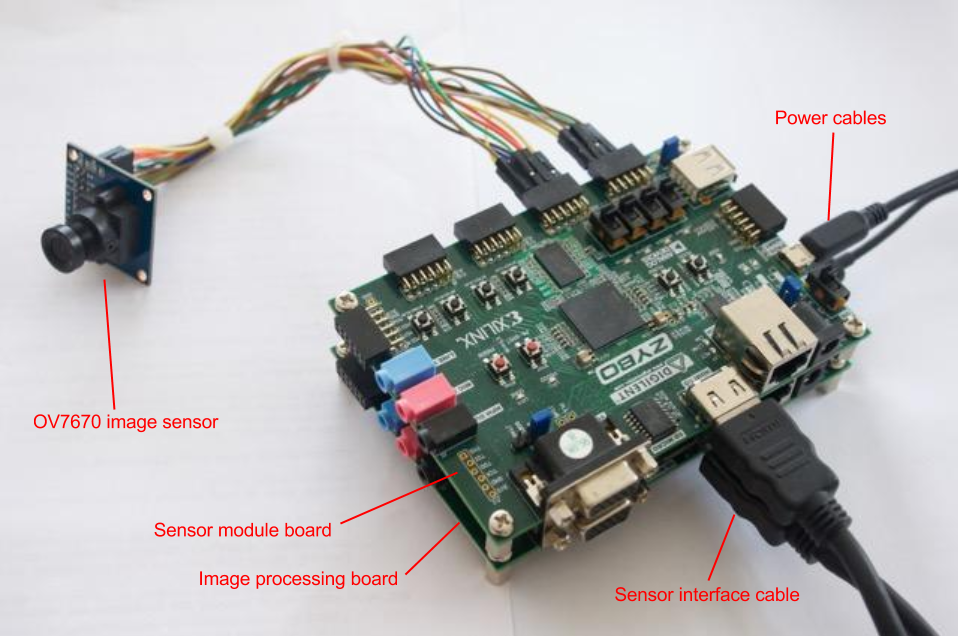
\includegraphics[width=1\textwidth]{./img/zybo_top.png}
  \caption{Finished proof-of-concept system.}
  \label{fig:zybo_top}
\end{figure}

\begin{figure}
  \centering
  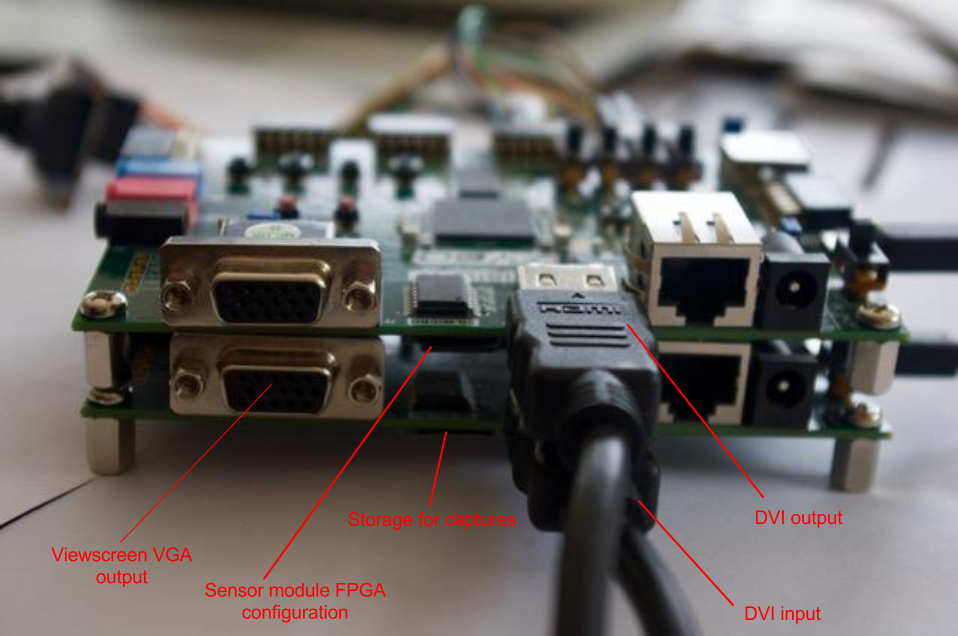
\includegraphics[width=1\textwidth]{./img/zybo_front.png}
  \caption{Image sensor interface connections and SD storage.}
  \label{fig:zybo_front}
\end{figure}
    
\section{Image capture}
The fundamental requirement for a camera system is that it can capture images. Using all of the parts specified in the design and implementation section, a proof-of-concept system has been built which can capture real-time video from a small 640 x 480 resolution image sensor, transmit them across a standardised interface to the main image processor, and store single frames on an external SD card.

Objective comparison of the whole system is fairly tricky as it requires comparing stills to another camera that uses an OV7670 image sensor in RAW mode. Instead, the analysis is done in two parts: the first part uses a test pattern generator to transmit a known image which we can compare pixel-for-pixel to the original, the second compares stills taken with the OV7670 to stills taken with a Pentax K-r \gls{dslr} set to an equivalent focal length.

All images taken with the proof-of-concept system were converted from \gls{pgm} to lossless PNG format using ImageMagick (\url{https://www.imagemagick.org}). As the image is captured as RAW data, the images have been post-processed on a computer using a linear interpolation de-mosaicing algorithm from MatLAB's Image Processing toolbox, as seen in Listing \ref{lst:matlab_demosaic}.

\begin{lstlisting}[caption={MatLAB's linear interpolation demosaicing algorithm.}, label={matlab_demosaic}, language=Matlab]
raw_img = imread('raw.png');
// Sensor CFA pattern:
// [B][G]
// [G][R]
colour_img = demosaic(raw_img, 'bggr');
imshow(colour_img);
\end{lstlisting}

\begin{figure}
\centering
\begin{subfigure}{.5\textwidth}
  \centering
  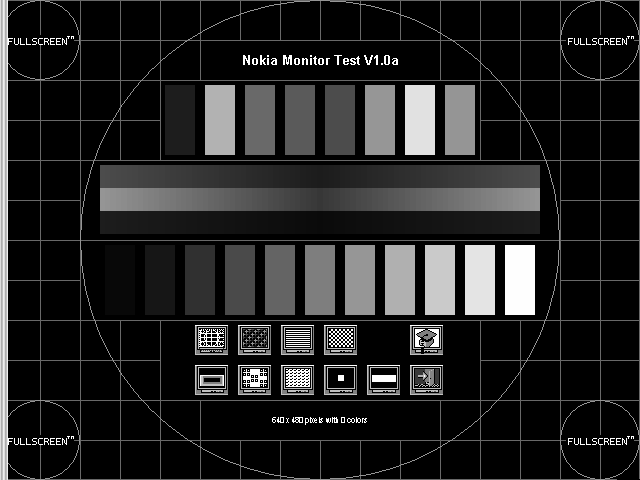
\includegraphics[width=.4\linewidth]{./img/ov7670_test_pattern_capture.png}
  \caption{Original test pattern stored in memory.}
\end{subfigure}%
\begin{subfigure}{.5\textwidth}
  \centering
  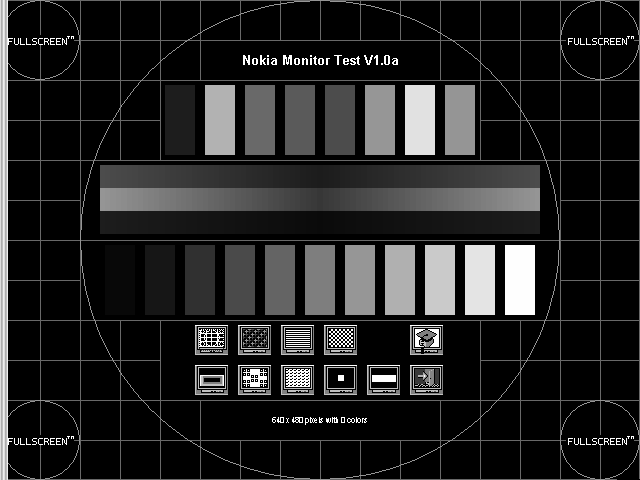
\includegraphics[width=.4\linewidth]{./img/ov7670_test_pattern_capture.png}
  \caption{Test pattern captured by image processor.}
\end{subfigure}
\label{fig:test_pattern_capture}
\caption{Comparison of original test pattern and image captured and saved by the image processor.}
\end{figure}

For Figure \ref{fig:test_pattern_capture}, a 640 x 480 resolution Nokia-provided test pattern normally used for testing monitors was loaded into the main framebuffer of the \gls{ps} on the sensor module board and transmitted over the image sensor interface at 72 \gls{fps} to the image processing board for storage on the SD card. When compared byte-for-byte, the two images are identical, meaning that the interface perfectly preserves the integrity of the data, thus it is a truly lossless interface.

\subsection{OV7670 stills}

Figures \ref{fig:lego_capture} and \ref{fig:texture_capture} show a comparison between images taken with a Pentax K-r \gls{dslr} and an OV7670; in addition two standalone Figures \ref{fig:ov7670_pcb} and \ref{fig:ov7670_spider} demonstrate macro photography with the OV7670. The first image in each set provides a reference image for the scene, however it should be noted that the colour balance and such has not been properly calibrated and thus cannot be used for a full objective comparison.

Immediately noticeable is that a vertical green line (appears as a black on the RAW capture) is present on every image capture from the OV7670. Also noticeable is a black line on the right-hand side and what appears at first glance to be a line of corrupted data of similar width on the left hand side. Given that the test patterns are the same resolution and are transmitted with all data in tact, it would seem that the image sensor and / or capture logic is at fault. To exclude the possibility of a faulty image sensor a second OV7670 was acquired and tested, however the data corruption was still evident. The most probably cause for this corruption is that the capture logic cannot properly synchronise with the start of the frame.

Images captured from the OV7670 tend to have a red / green hue to them as a result of poor colour balance. While the images from the Pentax K-r are not balanced either, they are visibly more neutral. Observing the colour histograms in Figure \ref{fig:lego_capture}, the OV7670's colour channels have a visible spread, raising the colour temperature and causing the highlights to have a red / green hue. The OV7670 was set up to adjust white balance automatically, but also provides registers to configure the white balance manually, which would allow for tighter control.

Figure \ref{fig:ov7670_spider} shows visible screen tearing issues. Significant lateral camera movement occurred as a result of the image being taken hand-held. Because only a single framebuffer is used, it is possible for the framebuffer readout to occur part way through being refreshed with new data from the sensor. The result is that the lower portion of the image contains stale data from before the camera moved, while the upper portion is from the current frame which hasn't been fully written out yet. The effect is only obvious when camera movement occurs. Double---or even triple---buffering is commonly used to reduce any screen tearing by writing new data to a second buffer, while drawing the first one to screen. Each frame the buffers are swapped so that the frame that was just written now gets drawn to the screen, and the frame which was just drawn gets overwritten with new data. While this would double the memory requirements, it would have no significant impact on performance and would vastly improve the image quality.

\begin{figure}
\centering
\begin{subfigure}{.5\textwidth}
  \centering
  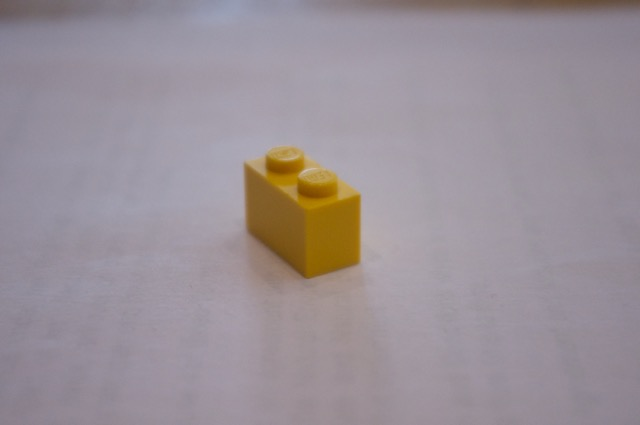
\includegraphics[width=.4\linewidth]{./img/pentax_lego.jpg}
  \caption{Pentax K-r}
\end{subfigure}%
\begin{subfigure}{.5\textwidth}
  \centering
  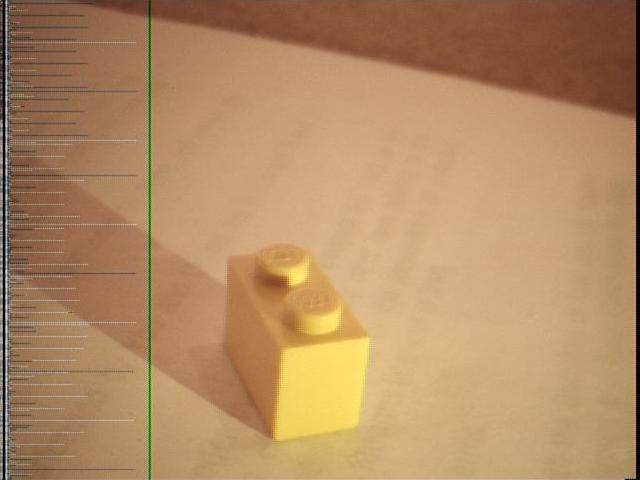
\includegraphics[width=.4\linewidth]{./img/ov7670_lego.jpg}
  \caption{OV7670}
\end{subfigure}
\begin{subfigure}{.5\textwidth}
  \centering
  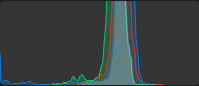
\includegraphics[width=.4\linewidth]{./img/pentax_lego_histogram.png}
  \caption{Pentax K-r histogram}
\end{subfigure}%
\begin{subfigure}{.5\textwidth}
  \centering
  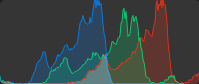
\includegraphics[width=.4\linewidth]{./img/ov7670_lego_histogram.png}
  \caption{OV7670 histogram}
\end{subfigure}
\label{fig:lego_capture}
\caption{Comparison test of yellow Lego brick.}
\end{figure}

\begin{figure}
\centering
\begin{subfigure}{.5\textwidth}
  \centering
  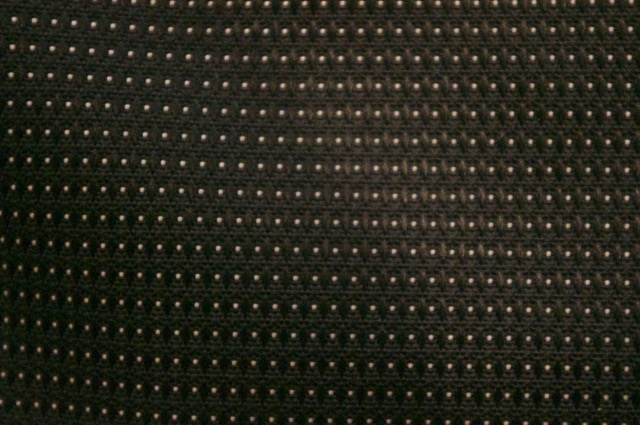
\includegraphics[width=.4\linewidth]{./img/pentax_texture.jpg}
  \caption{Pentax K-r}
\end{subfigure}%
\begin{subfigure}{.5\textwidth}
  \centering
  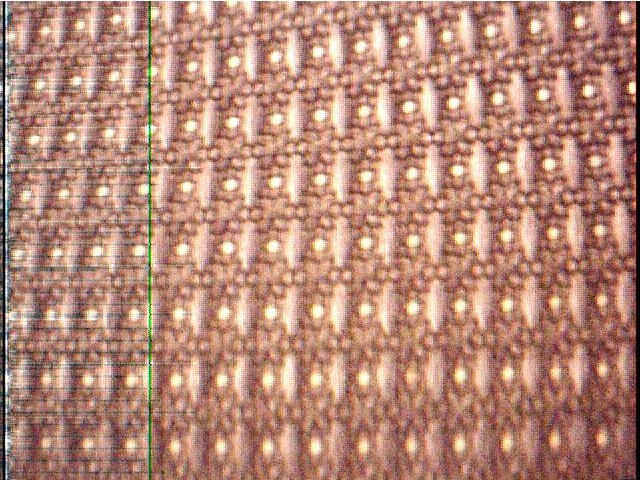
\includegraphics[width=.4\linewidth]{./img/ov7670_texture.jpg}
  \caption{OV7670}
\end{subfigure}
\label{fig:texture_capture}
\caption{Comparison test of repeated pattern.}
\end{figure}

\section{Soak testing}
To test continuous reliable operation of the interface, a test pattern generator was written to output incrementing bits (such that pixel 1 = 0, pixel 2 = 1, pixel 3 = 2...) at the pixel clock rate. Listing \ref{lst:test_pattern_generator} shows the code which generates an incrementing pattern to pass on to the \gls{dvi} encoder. A matching pattern checker was written (shown in Listing \ref{lst:pattern_checker}) and placed after the decoder to ensure that the received bit pattern was the same as that transmitted. Upon detecting a bit error an interrupt would be triggered on the \gls{ps} and an error message logged over the UART serial port. Listing \ref{lst:pattern_error} shows the firmware for the interrupt handler which logs an error message if a bit error occurs.

The test pattern generator was configured for 1080p output and connected to the HDMI output port on the sensor module board, which was connected via a HDMI cable to the HDMI input port on the image processor board, and fed into the \gls{dvi} decoder and then on to the pattern checker. The system was left running for twelve hours, with all serial port activity being logged. Apart from a single error when the two boards were initially powered on (caused by the two patterns needing to first synchronise), no other errors occurred during the twelve hour period. This is key in proving that the the design meets the requirements outlined in Table \ref{table:interface_specification} --- the interface is able to operate reliably for 12 hours at full HD resolution, transmitting at an aggregate rate of \SI{2.99}{\giga\bit\per\second}.

\begin{lstlisting}[caption={Test pattern generator outputs an incrementing bit pattern.}, label={lst:test_pattern_generator}, language=Verilog]
// Only increment counter pattern during non-blanking period
if (h_count < DISPLAY_WIDTH && v_count < DISPLAY_HEIGHT) begin
   counter <= counter + 1;
end

{b, g, r} <= counter;
\end{lstlisting}

\begin{lstlisting}[caption={Test pattern checker ensures the received bit stream is the same as that sent.}, label={lst:pattern_checker}, language=Verilog]
if (vde) begin
    if ((data != last_value + 1) && (data > 0)) begin
        error <= 1;
    end else begin
        error <= 0;
    end
    last_value <= data;
end else begin
    error <= 0;
end
\end{lstlisting}

\begin{lstlisting}[caption={Interrupt handler for bit pattern error.}, label={lst:pattern_error}, language=C]
static void ErrorHandler(void *callback_ref) {
    XTime now;
    XTime_GetTime(&now);
    xil_printf("Pixel error after %d seconds\n",
            (int) (1.0 * (now - start) / COUNTS_PER_SECOND));
}
\end{lstlisting}


%\section{Critical path}
%\section{Maximum throughput}
\section{Flash write speeds}

A significant bottleneck of the system is the flash storage. To test the system throughput files of varying sizes were written to an SD card attached to the Zybo development board. To ensure maximum performance all non-essential interrupts were disabled to ensure the Xilffs library was not blocked by anything else. Several different SD card variants (SD, SD High Capacity, SD eXtended Capacity) were tested, however neither the SDHC nor SDXC cards would were supported by the Xilffs library. Thus the results presented here are using a miscellaneous \SI{2}{\giga\byte} micro SD card from SanDisk.

Figures \ref{fig:standalone_write_graph} and \ref{fig:linux_write_graph} show the elapsed time for writing files of varying sizes to an SD card. 

\begin{figure}
  \centering
  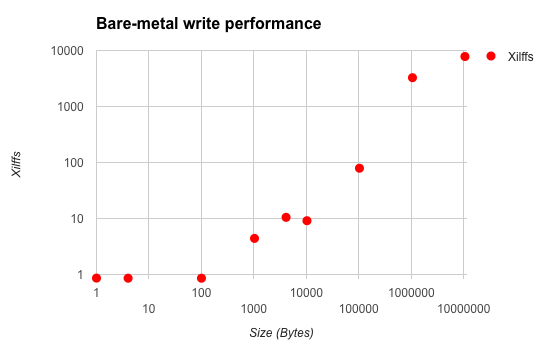
\includegraphics[width=1\textwidth]{./img/standalone_write_graph.png}
  \caption{SD write speeds using Xilffs on bare-metal system.}
  \label{fig:standalone_write_graph}
\end{figure}

\begin{figure}
  \centering
  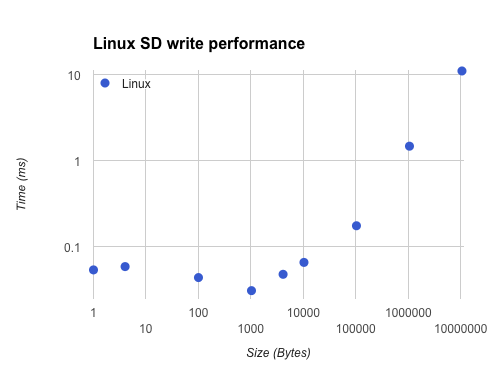
\includegraphics[width=1\textwidth]{./img/linux_write_graph.png}
  \caption{SD write speeds using embedded Linux kernel.}
  \label{fig:linux_write_graph}
\end{figure}


To store RAW video from the OV7670 at 30 \gls{fps} would require a sustained write speed of \SI{9.2}{\mega\byte\per\second}. The Xilffs library used by the bare-metal system has a very low maximum sustained throughput of \SI{1.3}{\mega\byte\per\second}, which would not meet the minimum requirements for video capture. The Linux FAT drivers on the other hand manage a maximum sustained throughput of around \SI{78}{\mega\byte\per\second}, which would be sufficient even for full HD video (although this would require some lossless compression to be used). An unfortunate side effect of the Xilinx FAT library is that it has the tendency to corrupt the filesystem. After completing the write performance testing, the SD card needed to be re-formatted as it was no longer recognised when plugged in to a computer. The Linux drivers on the other hand are very robust --- the SD card can be ejected mid-transfer without any damage to the filesystem.
